\documentclass[final]{article}

\makeatletter
\providecommand{\@trackname}{}
\makeatother
\usepackage{APS360}
\setcitestyle{numbers,square}
\usepackage[utf8]{inputenc}
\usepackage[T1]{fontenc}
\usepackage{hyperref}
\hypersetup{hidelinks}
\usepackage{url}
\usepackage{booktabs}
\usepackage{amsmath}
\usepackage{graphicx}
\usepackage{microtype}
\usepackage{xcolor}

\title{Frozen Regime Stress Tests for Cryptocurrency Direction Prediction}
\author{Bernie Fang\\1008726648, bernie.fang@mail.utoronto.ca\\
\href{https://github.com/Saberartoria77/APS-360-Project}{GitHub repository}}

\setlength{\textfloatsep}{7pt plus 1pt minus 2pt}
\setlength{\floatsep}{6pt plus 1pt minus 2pt}
\setlength{\intextsep}{6pt plus 1pt minus 2pt}
\newcommand{\tighthead}[1]{\vspace{0.25em}\noindent\textbf{#1}}

\begin{document}
\maketitle
\vspace{-3.8em}
\small

\section{Introduction}
\textbf{Main result.} A frozen CNN--LSTM attained prospective macro-F1 $0.409$ and accuracy $0.489$
on 1,488 genuinely unseen BTC/ETH forecast origins in July 2026. Its historical test macro-F1 was
$0.429\pm0.004$ across three seeds, and explicit regime transfer reduced macro-F1 by
$0.081\pm0.005$ (low$\rightarrow$high) and $0.057\pm0.005$ (high$\rightarrow$low). Thus the model
retained some balanced classification ability on new data but was not regime-invariant. Macro-F1 is
the unweighted mean of the three class F1 scores; accuracy is the overall correct fraction.

The goal is to predict whether the next-hour close return for BTCUSDT or ETHUSDT is \emph{down},
\emph{flat}, or \emph{up}, and to quantify how performance changes with volatility. This is difficult
and useful as a robustness study because crypto markets are noisy, imbalanced, and non-stationary.
Machine learning is appropriate for testing multivariate nonlinear temporal associations; convolution
can detect local motifs while an LSTM can retain longer dependencies. The study does not infer
causality or trading profitability.

\subsection{Related Work}
Fischer and Krauss benchmarked LSTMs against memory-free classifiers for equity direction and found
that performance varied across sub-periods \citep{fischer2018deep}. Nelson et al. used technical
indicators with an LSTM for stock movement classification \citep{nelson2017stock}, while Ghosh et
al. compared LSTMs and random forests on out-of-sample intraday directions
\citep{ghosh2020forecasting}. At cryptocurrency scale, Zhao modeled short-horizon movement from
trade-by-trade sequences \citep{zhao2021deep}. Guo et al. combined multiscale residual convolution
and LSTM components for Bitcoin price forecasting \citep{guo2021mrclstm}. These works motivate
sequence learning and simple baselines; this project instead emphasizes causal volatility slicing,
paired cross-regime transfer, three-seed uncertainty, and a pre-committed future month.

\begin{figure}[!h]
  \centering
  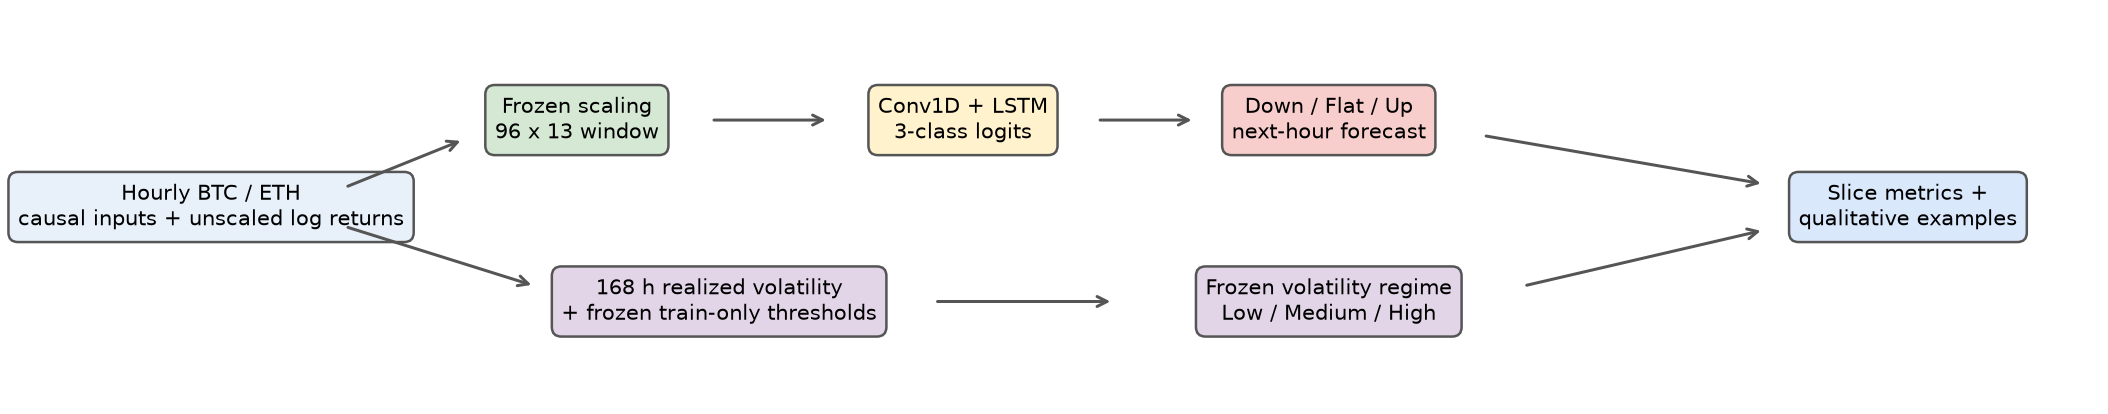
\includegraphics[width=0.99\linewidth]{artifacts/final/figures/model_regime_diagram.png}
  \caption{Two frozen paths share each forecast origin: a $96\times13$ sequence produces a
  three-class prediction, while trailing 168-hour realized volatility assigns a train-thresholded
  regime. Their outputs meet only during evaluation, preventing the next-hour outcome from defining
  its own regime.}
  \label{fig:pipeline}
\end{figure}

\newpage
\section{Data Processing}
Binance public hourly OHLCV klines cover July 1, 2023 00:00 UTC through June 30, 2026 23:00 UTC:
26,304 rows per asset (52,608 total). Timestamps were converted to UTC, sorted, deduplicated, and
required to be hourly contiguous. Thirteen causal features were computed: simple/log returns,
high--low range, close--open return, volume change, RSI(14), MACD(12,26,9), Bollinger position and
width(20), 24-hour volatility, and 24-hour volume z-score. A sample at forecast origin $t$ contains
the preceding 96 hourly feature rows through $t$; its label uses the close return from $t$ to $t+1$.
The training-only median absolute return, $0.2357\%$, defines down ($r<-0.2357\%$), flat, and up
($r>0.2357\%$).

Chronological 70/15/15 partitions yielded 36,584 training, 7,698 validation, and 7,702 historical
test windows. Training class counts were 8,838/18,230/9,516 (down/flat/up); historical test counts
were 2,061/3,703/1,938. Feature means/scales, label threshold, and model selection were fitted using
training or validation data only; no window crosses a symbol or split boundary.

\tighthead{Genuine example.} At BTCUSDT 2026-06-30 22:00 UTC, raw
open/high/low/close/volume were 58,639.99/58,806.91/58,513.80/58,607.99/274.43078.
The engineered one-hour return was $-0.000546$, RSI(14) was 38.365, and 24-hour volatility was
0.003793. The next close was 58,624.71, a return of $+0.000285$; because its magnitude was below
the frozen threshold, the resulting class was flat.

\tighthead{Volatility regimes.} For each asset, trailing realized volatility at $t$ is the population
standard deviation of 168 hourly log returns available through $t$. The low/high cut points are the
training-only 33rd/67th percentiles: BTC $0.00390/0.00512$ and ETH $0.00520/0.00674$.
Values at or below the lower cut point are low; values above the upper cut point are high; the rest
are medium. Per-asset thresholds avoid using asset identity as a volatility proxy.

\section{Architecture}
The 18,067-parameter PyTorch model applies same-padded Conv1D ($13\rightarrow32$, kernel 5), ReLU,
batch normalization, and 0.15 dropout to all 96 steps. A one-layer LSTM with 48 hidden units feeds
the last hidden state through 0.20 dropout and a $48\rightarrow3$ linear logit head. CrossEntropyLoss
uses inverse-frequency training weights $w_c=N/(3n_c)$ and consumes logits directly; Softmax is
applied only at inference. Adam ($10^{-3}$), batch size 256, gradient clipping at 1.0, at most 12
epochs, and validation-loss patience 3 were used. Seeds 42--44 quantify variation; minimum validation
loss selected seed 43 before prospective access.

\section{Baseline Models}
All baselines use identical windows and labels. \emph{Majority} predicts the most frequent training
class (flat). \emph{Momentum} maps the last observed return through the frozen class threshold.
Class-balanced multinomial \emph{logistic regression} uses the last 13-feature vector. These represent
a no-signal prior, a parameter-free heuristic, and a fast memory-free learned comparator.

\newpage
\section{Quantitative Results}
Table~\ref{tab:overall} reports the two final evaluation periods. Historical CNN values are
mean$\pm$population standard deviation over seeds 42--44; deterministic baselines and the frozen
prospective seed are single evaluations. Macro-F1 is primary because flat is the largest class.

\begin{table}[!h]
\centering
\footnotesize
\caption{Overall performance on the historical test ($n=7{,}702$) and prospective July 2026
($n=1{,}488$). Every value comes from the saved genuine result JSON.}
\label{tab:overall}
\begin{tabular}{lcccc}
\toprule
& \multicolumn{2}{c}{Historical test} & \multicolumn{2}{c}{Prospective July}\\
Model & Macro-F1 & Accuracy & Macro-F1 & Accuracy\\
\midrule
Majority & 0.216 & \textbf{0.481} & 0.243 & \textbf{0.573}\\
Momentum & 0.380 & 0.421 & 0.356 & 0.447\\
Logistic regression & \textbf{0.429} & 0.480 & 0.380 & 0.529\\
CNN--LSTM & $0.429\pm0.004$ & $0.450\pm0.005$ & \textbf{0.409} & 0.489\\
\bottomrule
\end{tabular}
\end{table}

Historically, the CNN matched logistic regression on macro-F1 but not accuracy. Its recalls were
$0.383/0.514/0.398$ (down/flat/up), more balanced than logistic regression's
$0.271/0.656/0.366$. In July, CNN recalls were $0.368/0.627/0.244$: up recall weakened, yet CNN
remained the strongest model by macro-F1. Majority accuracy rose only because 853/1,488 July labels
were flat, demonstrating why accuracy alone is misleading.

\begin{figure}[!h]
  \centering
  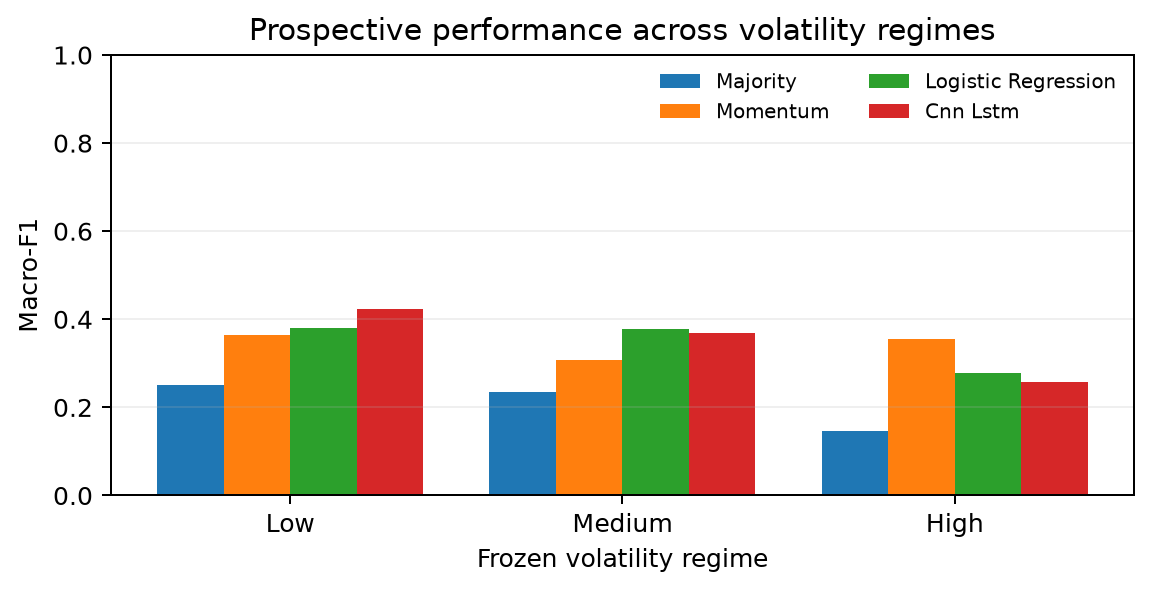
\includegraphics[width=0.70\linewidth]{artifacts/final/figures/regime_performance.png}
  \caption{Prospective macro-F1 under frozen regimes. CNN performance fell from 0.424 in low
  ($n=1{,}005$) to 0.368 in medium ($n=408$) and 0.258 in high volatility ($n=75$). The high-regime
  estimate is especially uncertain because that slice is small.}
  \label{fig:regimes}
\end{figure}

Figure~\ref{fig:regimes} shows a monotonic prospective deterioration for the CNN, but not every
baseline; the result supports sensitivity, not a universal causal effect of volatility. Historical
global CNN macro-F1 was 0.409/0.413/0.379 for low/medium/high ($n=2{,}033/3{,}240/2{,}429$).
More directly, CNNs trained only on low regimes scored $0.381\pm0.006$ on low versus
$0.300\pm0.001$ on high, a paired change of $-0.081\pm0.005$. High-trained CNNs scored
$0.409\pm0.005$ on high versus $0.352\pm0.001$ on low, a change of $-0.057\pm0.005$.
Logistic changes were $-0.063$ and $-0.071$. The consistent negative paired changes are the clearest
evidence of regime-dependent generalization.

\newpage
\section{Qualitative Results}
Examples were selected mechanically as the highest-confidence correct prediction and error in each
non-empty July regime, preventing editorial cherry-picking. In low volatility, the strongest correct
case was BTC flat at 88.6\% confidence (July 18 11:00 UTC), while the strongest error predicted flat
at 87.2\% for an actual BTC down move (July 25 04:00). Medium-regime examples repeated this pattern:
an 85.0\%-confidence correct flat and an 81.7\%-confidence false flat. In high volatility, confidence
was lower: an ETH down prediction was correct at 50.1\%, while another down prediction missed an up
move at 48.9\%. These cases align with the quantitative finding that the model can be confidently
biased toward flat in quieter periods and struggles to separate directions during rare high volatility.

\section{New Data}
The historical command trained all models, selected seed 43 by validation loss, froze CNN weights,
baselines, scaling, label/regime thresholds, feature order, and the exact July interval, and was
committed before July was fetched. Only then was the prospective command executed once. It used
June 24--30 solely as causal context and scored exactly 744 origins per asset from July 1 00:00
through July 31 23:00 UTC; the August 1 00:00 close resolves the last label. The 1,488 targets had
307/853/328 classes and 1,005/408/75 low/medium/high regimes. No prospective-dependent correction,
selection, retraining, or rerun was performed. The decline from historical CNN macro-F1 0.429 to
0.409 weakens the historical performance level, while its advantage over July baselines supports a
limited claim of prospective balanced classification. It does not establish profitability.

\section{Discussion}
The central finding is not that the hybrid model dominates: historically it only tied logistic
regression on macro-F1, and majority prediction won July accuracy. Rather, temporal modeling
distributed recall more evenly and achieved the best July macro-F1, while both explicit transfer and
the prospective regime slices exposed instability. The asymmetric errors are informative: low-trained
models lose flat recall in high volatility, whereas high-trained models transferred to low volatility
over-predict flat. This suggests distribution-specific class boundaries rather than a stable directional
mechanism. The project is challenging because returns are noisy, labels overlap around a learned
threshold, and both asset dynamics and class balance shift over time.

\tighthead{Limitations and future work.} Three seeds quantify optimization variability but not
sampling uncertainty; only two assets and one future month were tested, with just 75 high-volatility
July samples. Technical indicators omit order-book, macroeconomic, and sentiment information.
Future work should register multiple future months, add confidence intervals or block-bootstrap tests,
study calibration, and compare rolling retraining under a pre-declared protocol. Any trading study
would separately require fees, slippage, latency, and risk controls.

\section{Ethical Considerations}
Forecasts can encourage overconfidence, speculative losses, or unequal harm to users who cannot
absorb volatility. Binance data may not represent other venues, outages, liquidity, or manipulation;
historical patterns can fail abruptly. The system must be presented as an educational robustness
study, with uncertainty and failure cases visible, not as financial advice. Reproducible frozen
artifacts reduce selective reporting, but they do not make the predictions safe for deployment.

\clearpage
\bibliographystyle{plainnat}
\bibliography{refs}

\end{document}
